\chapter{Literature Review}

\section{Evolution of Time Series Forecasting} % Section 2.1


Nowadays \textbf{Time series forecasting} has become one, if not the most, crucial tool used in decision-making and strategic planning processes across a wide range of industries such as finance, economics, environmental science, and healthcare \cite{article}. The extensive use of time series analysis in many different industries can be attributed to its ability in examining past data, detecting hidden pattern, trends and seasonality and providing insightful forecasts, which is particularly important for the businesses in order to react and prepare for upcoming events. The methodologies used has changed considerably over the years thanks to the technological innovation, in  particular, the key drivers that have spurred the progress in time series analysis have been the increase of data availability and data volume, which have been pushed by the the rise of social media, Internet of Things (IoT), and multimedia, along with the growth of cloud computing, a powerful technology that enables to perform massive-scale and complex computing eliminating the need to purchase and maintain expensive computing hardware, dedicated space, and software\cite{HASHEM201598}.
The history of time series analysis goes back to the late 19th century, with the foundational work of Francis Galton and Karl Pearson on correlation, which then posed the basis for \textbf{George Udny Yule}, a British statistician, to further advance this concepts, developing the idea of regression between two variables X and Y, without relying on the assumption that the two variables were jointly normally distributed \cite{l_kristensen_foundations_2021} and its first known application was in his 1927 with the analysis of sunspots \cite{SILVERMAN198899}, in this paper Yule developed what is now known as an autoregressive time series analysis in order to estiamate the number of sunsposts for a given year as a function of the sunspots of the two preceding years and a presumed random disturbance. This fist model was a building block for the \textbf{ARIMA} (Autoregressive Integrated Moving Average) model, later developed in the 1970s by two mathematicians, George Box and Gwilym Jenkins, in a publication called "Time Series Analysis: Forecasting and Control", with the objective of capturing the underlying patterns in time series data leveraging the three components that compose the model: autoregression, integrated, moving average. \cite{article_2}. The ARIMA model has gained a lot of popularity in the past and was one of the most commonly used approach to time series modeling as they take both long-term trends and sudden shocks into account, and many different variations where developed, to deal with the limitations of the original one, namely the ARIMAX, SARIMA, SARIMAX, VARIMA and VARIMAX models. In modern times, although ARIMA models are still being used, they are considered "classical" approaches and with the technological and statistical advancement new techniques and algorithms have been developed, capable of handling more complexed, high-dimensional, non linear time series data, leveraging machine learning and deep leaning models.


\subsection{Classical Models}  % (ARIMA, SARIMA, GARCH)}  Subsection 2.1.1
\subsubsection{ARIMA models}
An \textbf{ARIMA} (Autoregressive Integrated Moving Average) model, it's a more sophisticated extension of the simpler \textbf{ARMA} (Auto Regressive Moving Average) model, which combines two concepts: AR (Auto Regressive) and MA (Moving Average). 

\textbf{AR model}

Autoregressive models are regression models applied on lag series generated using the original time series. In mulitivariate linear regression, the output, the dependendent variable, is expressed as linear combination of multiple independent variables: \( y = \beta_0 + \beta_1 x_1 + \beta_2 x_2 + \cdots + \beta_n x_n + \epsilon \).
Similarly in autoregressive models with p lags or an \textbf{AR(p)} models the output (the future data point) can be expressed as a linear combination of the past p data points, where p represent the lag window: 
\begin{equation}
 y_t = \phi_1 y_{t-1} + \phi_2 y_{t-2} + \cdots + \phi_p y_{t-p} + \epsilon_t 
\end{equation}
Autoregressive models, in order to be applied, require time series to be \textbf{stationary}, which means that the statistical properties of the series, such as its mean, variance, and auto-covariance, remain constant over time. Otherwise non-stationary data can lead to unreliable model outputs and inaccurate predictions. Practically this imposes certain restrictions on the values of the autoregressive coefficients, which implies that the roots of the characteristic equation:
\begin{equation}
 1 - \phi_1 z - \phi_2 z^2 - \ldots - \phi_p z^p = 0
\end{equation}
must lie outside the unit circle, (\(|z_i| > 1 \quad\)for all roots \(z_i)\)) \cite[Section 3.2]{box1970time}.

\begin{figure}[H]
    \centering
    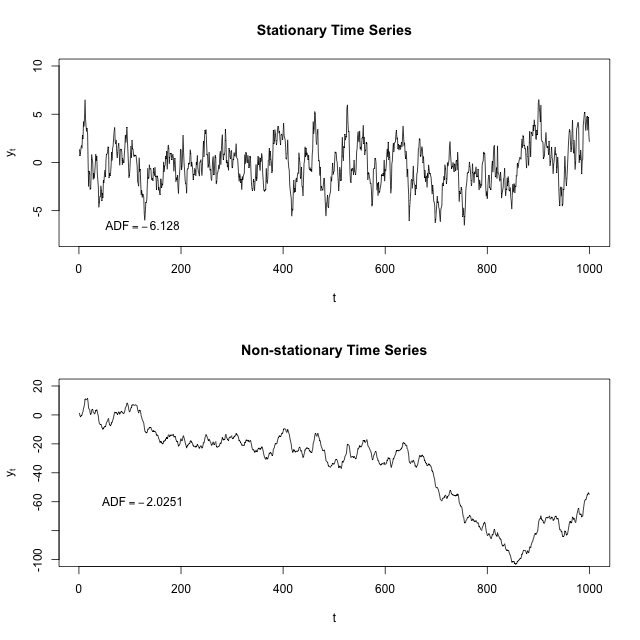
\includegraphics[width=0.50\textwidth]{Machine_learning_thesis/Images/Stationarycomparison.png}
    \caption{Example of a stationary and non-stationary process.} 
    \label{fig:Stationarycomparison}
\end{figure}

\textbf{MA model}

A moving average model uses past forecast errors in a regression-like model to predict an output(future data point), in particular, in a moving average model of order q, \textbf{MA(q)}, the ‘q’ parameter represents the number of lagged error terms to be considered in the model equation:
\begin{equation}
y_t = \mu + \varepsilon_t + \theta_1 \varepsilon_{t-1} + \theta_2 \varepsilon_{t-2} + \cdots + \theta_q \varepsilon_{t-q}
\label{MA equation}
\end{equation}
Contrary to AR(p) models, MA(q) models are stationary for any values of the coefficients \cite{chatfield2009}, indeed, if we consider the equation of a MA(q) model \eqref{MA equation}, \(y_t\) is essentially a linear combination of present and past values of \(\varepsilon_{t}\), which are assumed to be independent and identically distributed random variables with mean of zero and constant variance \( \sigma^2\), whose terms are uncorrelated. Nevertheless some constraints on the parameters of the models should be applied anyway to ensure that the model is \textbf{invertible}, which means that it can be algebraically equivalent to a converging infinite order AR model, AR(\(\infty\)), this ensure that it exists a unique MA process for a given autocorrelation function \cite{chatfield2009}. Practically this is achieved if the roots of the characteristic equation: 
\begin{equation}
 1 - \phi_1 z - \phi_2 z^2 - \ldots - \phi_p z^p = 0
\end{equation}
all lies outside the unit circle,(\(|z_i| > 1 \quad\)for all roots \(z_i)\)) \cite[pag. 50] {box1970time}.

\textbf{ARMA model}

An \textbf{ARMA(p,q)} model simply merges the two previously described models, therefore it can be expressed as: 
\begin{equation}
y_t = \mu + \phi_1 y_{t-1} + \theta_1 \epsilon_{t-1} + \epsilon_t
\end{equation}
where p and q are respectivelly the orders of the AR and MA models.

\textbf{ARIMA model}

In practise, the majority of real world time series are not stationary, and thus they must often be transformed in order to make them stationary. An \textbf{ARIMA(p, q, d)} model it's a generalizations of the autoregressive moving average (ARMA) model to non-stationary series and periodic variation with the addition of an integration component, denoted with \textbf{I(d)}, which helps  remove trends and stabilize the series in the mean sense (but it does not affect the non-stationarity of the variance or autocovariance) \cite{chatfield2009}. This can be done by differencing, which involves subtracting the preceding observation from the current one, mathematically:
\begin{equation}
 y'_t = y_t - y_{t-1}
\end{equation}
This operation is known as "first differencing",  \(\Delta\), and it is often sufficient to eliminate linear trends and achieve stationarity. If the series still shows trends or non-stationary behavior after the first pass through this process, applying "second differencing", \(\Delta^2\), may help. 
\begin{equation}
 y_t'' = (y_t - y_{t-1}) - (y_{t-1} - y_{t-2}) = y_t - 2y_{t-1} + y_{t-2}
\end{equation}
The total number of differencing is determined by the parameter d, which typically assumes the values 0, 1, 2 as higher differencing can remove too much informations from the data, over-complicating the model. The generalized  ARIMA (Autoregressive Integrated Moving Average) model can be expressed mathematically as \cite{Hung2023}: 
\begin{equation}
y_t = c + \phi_1 y_{t-1} + \cdots + \phi_p y_{t-p} + \theta_1 \epsilon_{t-1} + \cdots + \theta_q \epsilon_{t-q} + \epsilon_t
\label{ARIMA equation}
\end{equation}
which can be rewritten using backshift notation as:
\begin{equation}
\Phi(B^d)(y_t - \mu) = \Theta(B)\epsilon_t
\end{equation}
where: 
\begin{itemize}

    \item \( B \) is the backshift operator such that \( B^k y_t = y_{t-k} \).
    \item \( \Phi(B^d) \) is the autoregressive polynomial of order \( p \) given by: \(\Phi(B^d) = 1 - \phi_1 B - \phi_2 B^2 - \ldots - \phi_p B^p\)
    \item \( \Theta(B) \) is the moving average polynomial of order \( q \) given by: \(\Theta(B) = 1 + \theta_1 B + \theta_2 B^2 + \ldots + \theta_q B^q\)
\end{itemize}

This model was introduce for the fist time in 1970, when the statisticians George Box and Gwilym Jenkins proposed what has become known as the Box-Jenkins method \cite{box1970time}, an approach that outlines a systematic way to identify and fit an ARIMA model to specific time series data.
\begin{figure}[H] 
    \centering
    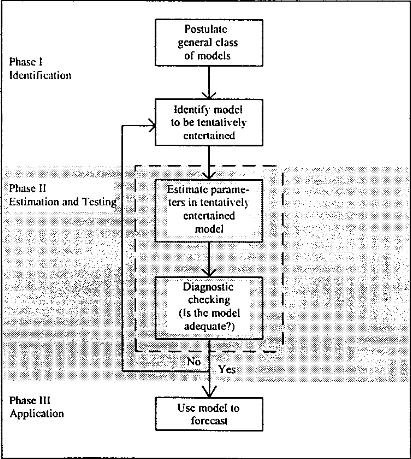
\includegraphics[width=0.4\textwidth]{Machine_learning_thesis/Images/Box_Jenkins_methodology.png}
    \caption{Schematic representation of the Box-Jenkins methodology.} 
    \label{fig:box_jenkins_methodology} 
\end{figure}

The original model used an iterative three-stage modeling approach:
\begin{enumerate}
    \item \textbf{Model Identification and Selection}: ensure the variables are stationary and identify the dependent variable's seasonality (if necessary, apply seasonal differencing). Use the plots of autocorrelation (ACF) and partial autocorrelation (PACF) functions of the dependent time series to determine which autoregressive or moving average components to use in the model.
    \item \textbf{Parameter Estimation}: utilize computation algorithms to derive the coefficients that best fit the selected ARIMA model. The most common methods for estimation are maximum likelihood estimation or non-linear least-squares estimation.
    \item \textbf{Statistical Model Checking}: test whether the estimated model conforms to the specifications of a stationary univariate process:  the residuals should be independent of each other and their mean and variance constant over time. Helpful techniques for identifying model misspecification include:
    \begin{itemize}
            \item Plotting the mean and variance of residuals over time.
            \item Performing a Ljung–Box test.
            \item Plotting the autocorrelation and partial autocorrelation of the residuals.
    \end{itemize}
    \item \textbf{Model Refinement}: if the estimation is inadequate, return to step one and attempt to build a better model.
\end{enumerate}

In empirical studies however it appears that the accuracy of such models is generally worse than much simpler time series methods. The major problem lies in the way of making the series stationary in its mean that has been proposed by Box and Jenkins. If alternative approaches are utilized to remove and extrapolate the trend in the data, ARMA models outperform the models selected through Box–Jenkins methodology \cite{Smith1997}. 

\textbf{SARIMA model}

ARIMA models do not support seasonal data, which are time series characterised by periodic fluctuations that repeats over a certain period (e.g. monthly, quarterly, yearly).
\begin{figure}[H] 
    \centering
    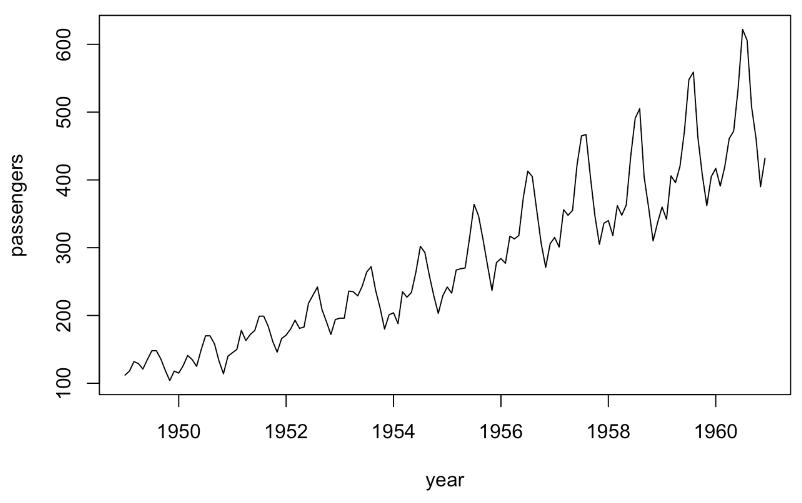
\includegraphics[width=0.4\textwidth]{Machine_learning_thesis/Images/Monthly Air Passengers(1949 - 1960).png}
    \caption{Example of a time series with seasonality (Monthly Air Passengers(1949 - 1960) Time Series).} 
    \label{fig:time_series_seasonality} 
\end{figure}
Seasonal Auto-Regressive Integrated Moving Average models, \textbf{SARIMA(p, d, q)(P, D, Q)m}, are an extension of the ARIMA (Autoregressive Integrated Moving Average) model that incorporates seasonality, by including additional seasonal terms in the ARIMA model, which are denoted by (P, D, Q)m, which represent:
\begin{itemize}
    \item P: seasonal autoregressive order
    \item D: seasonal difference order
    \item I: seasonal moving average order
    \item m: number of timesteps for a seasonal period
\end{itemize}

The general SARIMA model can be represented mathematically as follows \cite{Lee2023}:
\begin{equation}
\phi_p(B)\Phi_P(B^s)W_t = \theta_q(B)\Theta_Q(B^s)\omega_t 
\end{equation} 
where: 
\begin{itemize}
    \item \( B \): is the backshift operator, defined as \( B^k Y_t = Y_{t-k} \) 
    \item \(\phi_p(B)\): is the non-seasonal autoregressive (AR) polynomial of order p given by: \(\phi_p(B) = 1 - \phi_1 B - \phi_2 B^2 - \cdots - \phi_p B^p\)
    \item \(\Phi_P(B^s)\): is the seasonal autoregressive (SAR) component of order P given by: \(\Phi_P(B_s) = 1 - \Phi_1 B_s - \Phi_2 B_{2s} - \cdots - \Phi_P B_{Ps}\) 
    \item \(W_t\): represents the observed time series at time t. 
    \item \(\theta_q(B)\): is the \textbf{non-seasonal moving average (MA)} component of order q, give by : \(\theta_q(B) = 1 + \theta_1 B + \theta_2 B^2 + \ldots + \theta_q B^q\)
    \item \(\Theta_Q(B^s)\): is the seasonal moving average (SMA) component of order Q, given by: \(\Theta_Q(B_s) = 1 + \Theta_1 B_s + \Theta_2 B_{2s} + \ldots + \Theta_Q B_{Qs}\)
    \item \(\omega_t\): is the white noise error term at time t
\end{itemize}

\subsubsection{ARCH/GARCH}
Traditional time series models, like ARIMA models, assume costant variance over time, \textbf{homoskedasticy} \cite{MeatPrices2023}, indeed, if we look back at the formula of the ARIMA model \eqref{ARIMA equation},  \(\epsilon_t\), the white noise error term at time t is assumed to be normally distributed with mean zero and constant variance, mathematically: 
\begin{equation}
\text{Var}(\epsilon_t) = \sigma^2 \quad \text{for all } t
\end{equation}
However economic time series often shows \textbf{heteroscedasticity}, non-constant variance, that's beacuse  positive and negative news affect the variance
differently, which is known as the leverage effect. Addittionaly, economic time series often exhibit a behavior that is known as \textbf{volatility clustering}, where the volatility changes over time and its degree shows a tendency to persist. As a consequence, the dispersion of residuals changes over time, resulting in clusters of varying volatility rather than a constant spread.
\begin{figure}[H] 
    \centering
    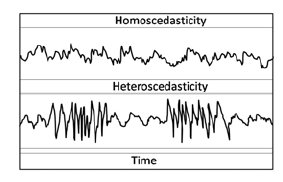
\includegraphics[width=0.5\textwidth]{Machine_learning_thesis/Images/Homoscedastic-vs-Heteroscedastic.png}
    \caption{Homoscedastic vs Heteroscedastic time series.} 
    \label{fig:Homoscedastic-vs-Heteroscedastic} 
\end{figure}
For this reason in 1982 Autoregressive Conditional Heteroscedasticity (\textbf{GARCH}) model was introduced by Robert Engle \cite{Engle1982}, to account for variance changes in financial time series by modeling the variance as a time-varying process, dependent on past errors. 

\textbf{ARCH model}

An \textbf{ARCH(p)} model is essentially an AR(p) model applied to the \textbf{conditional variance} of a time series, where p represent the order of the model, the number of past time periods used to predict the current variance at time \(t\). The conditional variance represent the variance at time \(t\), given the information of the variance untill time \(t-1\) , mathematically it is a combination of the unconditional variance and the deviation of squared error from its average value . For an ARCH(p) model it  can be represented by the following equation \cite{PalombaGARCH}: 
\begin{equation}
\displaystyle \sigma _{t}^{2}=\alpha _{0}+\alpha _{1}\epsilon _{t-1}^{2}+\cdots +\alpha _{q}\epsilon _{t-q}^{2}=\alpha _{0}+\sum _{i=1}^{q}\alpha _{i}\epsilon _{t-i}^{2}
\end{equation} 
Where:
\begin{itemize}
    \item $\sigma_{t}^{2}$ is the conditional variance at time $t$.
    \item $\epsilon _{t-i}^{2}$ are the squared residuals from previous periods.
    \item $\alpha_{0}, \dots, \alpha_{p}$ are the parameters of the model and measure the sensitivity of the conditional variance $\sigma_{t}^{2}$ to past squared residuals.
\end{itemize}

Even though conditional variance changes over time, the model can be \textbf{covariance stationary} if the variance of the process stays finite and constant over time. For an ARCH(p) model, this happenswhen the roots of the polynomial $1-A(L)$ fall outside the unit circle, this translates to the condition \cite{PalombaGARCH}: 
\begin{equation}
\sum_{i=1}^{p} \alpha_{i} < 1
\end{equation} 
where:
\begin{itemize}
    \item A(L): is the lag polynomial: \(\alpha_1 L + \alpha_2 L^2 + \cdots + \alpha_q L^q\) 
    \item L is the \textbf{lag operator}, which shifts values of the time series back by a certain number of periods 
\end{itemize}

This will ensure that shocks to the system will be dissipated instead of accumulating over time, maintaining a bounded variance and ensuring that the unconditional variance exists, assuming this value: 
\begin{equation}
\text{Var}(\epsilon_t) = \frac{\alpha _{0}}{1 - \sum_{i=1}^{q} \alpha_i}
\end{equation} 


\textbf{GARCH model}

In practice, only rather rich ARCH parameterizations are able to fit financial series adequately, however, largely parameterized models can be difficult to estimate and can bring to instability during forecasting. The Generalized Autoregressive Conditional Heteroskedasticity (GARCH) model was introduced by Tim Bollerslev in 1986 \cite{Bollerslev1986} and expands upon the ARCH model by enabling a more parsimonious approach to analyzing time-varying volatility in financial series without estimating an overly complex parameter structure. 

Unlike ARCH, which uses an autoregressive model of the past squared errors to capture volatility, the GARCH model extends this by adding the past conditional variance alongside the past squares. This is represented as a \textbf{GARCH(p, q)} model, where p and q are orders for the autoregressive and moving average terms in the variance equation, respectively. The general form for the conditional variance, \(\sigma _{t}^{2}\) , in a GARCH(p, q) model is:
\begin{equation}
\sigma_{t}^{2} = \alpha_{0} + \sum_{i=1}^{p} \alpha_{i} \epsilon_{t-i}^{2} + \sum_{j=1}^{q} \beta_{j} \sigma_{t-j}^{2}
\end{equation} 
Where: 
\begin{itemize}
    \item $\alpha_{i}$ coefficients scale past squared error terms $\epsilon_{t-i}^{2}$.
    \item $\beta_{j}$ coefficients scale past conditional variances $\sigma_{t-j}^{2}$.
\end{itemize}

The GARCH(p, q) model is covariance stationary when the roots of the polynomial \(1 - A(L) - B(L)\) fall outside the unit circle. This results in the following condition: 
\begin{equation}
\sum_{i=1}^{q} \alpha_{i} + \sum_{j=1}^{p} \beta_{j} < 1
\end{equation} 
with all parameters \(\alpha_{0}, \alpha_{i}, \beta_{i}\) being non-negative. When this condition holds, the unconditional variance of the innovation is: 
\begin{equation}
\operatorname{Var}(\epsilon_{t}) = \frac{\omega}{1 - \sum_{i=1}^{q} \alpha_{i} - \sum_{j=1}^{p} \beta_{j}}
\end{equation}


\subsection{Machine Learning models} % (Random Forest, XGBoost, LightGBM)} Subsection 2.1.2
\subsubsection{Random Forest}
\label{Sec: Random Forest}
A Random Forest model, also referred to as Random Decision Forest, is an ensemble learning model (which will be discussed in more details in the section \ref{Sec: ensemble learning}), introduced for the first time by Ho in 1995 \cite{Ho1995}, however it was Breiman who significantly advanced the methodology in 2001 \cite{Breiman2001} publishing a version that is modified and being currently used. The model developed by Leo Breiman consists of a group of un-pruned classification or regression trees made from the random selection of samples of the training data. Random features are selected in the induction process. Prediction is then made by aggregating (majority vote for classification or averaging for regression) the predictions of the ensemble. Each tree is grown as described:
\begin{itemize}
\item \textbf{Random Sampling with Replacement}: N instances will be randomly sampled from the original dataset, with replacement, meaning that some instances may appear multiple times in a single sample, while others may be omitted. This sample will then be used as the training set for growing the tree.
\item \textbf{Random Feature Selection (Feature Bagging)}: For M input variables, a subset of features m is selected (such that $m<<M$) at each split for each tree, the best split will be then selected using the m features instead of the whole M input variables. This will reduce the correlation between trees making the ensemble more robust to noise.
\item \textbf{Tree Growth Without Pruning}: each tree is grown to the largest possible extent and no pruning is used.
\end{itemize}

Random Forest generally exhibits a significant performance improvement compared to a single decision tree \cite{Sharma2015}. 

\textbf{Regression tree}

Regression trees are obtained using a \textbf{greedy}, divide and conquer algorithm that recursively partitions the given training data into smaller subsets, to minimize the prediction errors. This process, also referred to as \textbf{top-down induction} of decision trees can be described by the following procedure: 
\begin{tcolorbox}[colback=blue!5, colframe=blue!80, colframe=white, boxrule=0pt]
\begin{algorithm}[H]
    \caption{Top-down induction of decision trees}
    \label{alg:tree_construction}
    \begin{enumerate}
        \item In the initialization phase, each observation is placed in the root node of the tree. The root is included in the list \( L \) of active nodes.
        \item If the list \( L \) is empty, the procedure is stopped; otherwise, a node \( J \) belonging to the list \( L \) is selected, removed from the list, and used as the node for analysis.
        \item The optimal rule to split the observations contained in \( J \) is then determined, based on an appropriate preset criterion. The splitting rule generated in this way is then applied, and descendant nodes are constructed by subdividing the observations contained in \( J \). 
        \begin{enumerate}
            \item For each descendant node, the conditions for stopping the subdivision are verified. 
            \item If these conditions are met, node \( J \) becomes a leaf and the value assigned to it is the mean of the target values of the observations contained in \( J \). 
            \item Otherwise, the descendant nodes are added to the list \( L \). Finally, step 2 is repeated.
        \end{enumerate}
    \end{enumerate}
\end{algorithm}
\end{tcolorbox}

The procedure above is a general framework and requires some additional steps to be specified before deriving an implementable regression algorithm:
\begin{itemize}
    \item \textbf{Splitting Rules:} For each node of the tree, it is necessary to specify the criteria used to identify the optimal rule for splitting the observations and for creating the descendant nodes. There are several alternative criteria, which differ in the number of descendants, the number of attributes, and the evaluation metrics.
    \item \textbf{Stopping Criteria:} At each node of the tree, different stopping criteria are applied to establish whether the development should be continued recursively or if the node should be considered a leaf. Various criteria have been proposed for this purpose, resulting in quite different topologies of the generated trees, even if all other elements are held constant.
    \item \textbf{Pruning Criteria:} Finally, it is appropriate to apply pruning criteria to avoid excessive growth of the tree during the development phase (\textit{pre-pruning}) and to reduce the number of nodes after the tree has been generated (\textit{post-pruning}).
\end{itemize}

The trees that are usually employed in Random Forest models are \textbf{binary}, \textbf{univariate} decision trees (as described in the following papers \cite{Cutler2011}, \cite{Bernard2009}, \cite {Geurts2006}) as they offer a good balance between interpretability and predictive accuracy, and help prevent overfitting in noisy or high-dimensional datasets. These trees partition the predictor space using a sequence of binary partitions (“splits”) on individual variables.
\begin{figure}[H] 
    \centering
    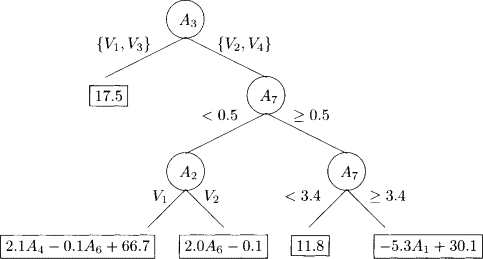
\includegraphics[width=0.5\textwidth]{Machine_learning_thesis/Images/regression tree.png}
    \caption{Example of a regression tree.} 
    \label{fig:Regression tree} 
\end{figure}
For a continuous predictor variable, a split is determined by a split-point; points for which the predictor is smaller than the split-point go to the left, the rest go to the right. 
\begin{figure}[H] 
    \centering
    \begin{tikzpicture}
        \node[anchor=center] (img) {
            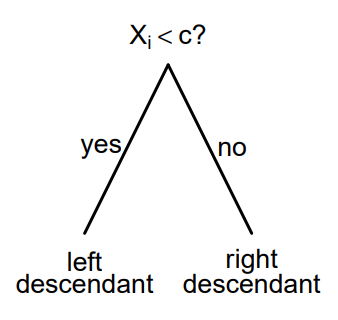
\includegraphics[width=0.3\textwidth]{Machine_learning_thesis/Images/Continuous variable split.png}
        };
        % Overlay a semi-transparent white rectangle
        \fill[white, opacity=0.2] (img.south west) rectangle (img.north east);
    \end{tikzpicture}
    \caption{Splitting on a continuous predictor variable $X_i$, using split-point $c$.} 
    \label{fig:split of a continuous variable} 
\end{figure}
The criterion used to determined the best split is the maximization of the \textbf{information gain},  $\Delta$, which is defined as: 
\begin{equation}
\Delta(q, q_1, q_2, \ldots, q_K) = I(q) - I(q_1, q_2, \ldots, q_K) = I(q) - \sum_{k=1}^{K}\frac{Q_k}{Q} I(q_k)
\end{equation}
Where: 
\begin{itemize}
    \item $I(q)$: represent the impurity index of the parent node
    \item $I(q_1, q_2, \ldots, q_K)$: represent the impurity index of the split, which is equal to the weighted sum of the impurities of each descendant node (which in the context of binary trees will be two), where each weight equals to the percentage of examples from the parent node that are placed in the corresponding descendant.  
\end{itemize}

The \textbf{heterogeneity index} (or impurity index) $I(q)$ of a node for a regression tree is a function of the variability of the target values for the examples at the node, and it has to satisfy three requirements: 
\begin{itemize}
    \item it must take its maximum value when the examples at the node are distributed homogeneously with respect to the target variable.
    \item it must take its minimum value when all the instances at the node assume the same target value.
    \item it must be a symmetric function with respect to the distribution of target values in the node.
\end{itemize}

A measure of the heterogeneity index, for regression trees, is the mean squared error: 
\begin{equation}
    I(q) = \sigma^2 = \frac{1}{N} \sum_{i=1}^{N} (y_i - \bar{y})^2
\end{equation}
Although pruning is important to prevent over-fitting for stand-alone trees, it is not used in Random Forests.

\textbf{Random Forest}
As mentioned before at the beginning of section \ref{Sec: Random Forest}, a Random Forest uses trees as base learners. Random forests are based on the concept of \textbf{bagging}, where each tree is fit to an independent \textbf{bootstrap sample} from the original data and the final prediction is obtained by averaging the results of each tree's prediction. Random Forest enhance bagging by introducing an additional level of randomness: when splitting a node, the best split is found over a randomly selected subset of $m$ predictor variables instead of all $M$ predictors, independently at each node. Two notable variations of this idea include \textbf{Forest-RI} (Random Input selection) and \textbf{Forest-RC} (Random Linear Combination selection):
\begin{itemize}
    \item Forest-RI: it randomly selects at each node, $m << M$ attributes ($m$ is fixed) as candidates for the split at the node. There is still correlation between the trees because they are based on the same observations. 
    \item Forest-RC: it represent a more radical approach, instead of using the original attributes, this method performs a perturbation which is even greater than the original dataset. It creates new attributes that are random linear combination of the existing attributes. In this way it is possible to reduce the correlation between the individual classifiers/trees. 
\end{itemize}

The process can be summirez by the following algorithm:
\begin{tcolorbox}[colback=blue!5, colframe=blue!80, boxrule=0pt]
    \begin{algorithm} [H]
        \caption{Random Forest}
        \label{alg:random_forest}
        Let $\mathscr{D} = {(x1, y1),...,(xN, yN)}$ denote the training data, with $xi = (xi,1,..., xi,p)^T$. 
        For $j = 1$ to $J$:
        \begin{enumerate}
            \item Take a bootstrap sample $\mathscr{D}_j$ of size $N$ from $\mathscr{D}$.
            \item Using the bootstrap sample $\mathscr{D}_j$ as the training data, fit a tree using binary recursive partitioning (Algorithm \ref{alg:tree_construction}).
            \begin{enumerate}
                \item Select m predictors at random from the p available predictors.
                \item Find the best binary split among all binary splits on the m predictors from step (a).
                \item Split the node into two descendant nodes using the split from step (b).
            \end{enumerate}
            \item Make a prediction at a new point $x$: 
            \[
                \hat{f}(x) = \frac{1}{J} \sum_{j=1}^{J} \hat{h}_j(x)
            \]
        \end{enumerate}
    \end{algorithm}
\end{tcolorbox}

\subsubsection{}


\subsection{Advances in Deep Learning} %(LSTM, GRU, CNN)} Subsection 2.1.3
% Content for deep learning models

\section{Modern Ensemble Techniques in Time Series} % Section 2.2
\label{Sec: ensemble learning}

\subsection{Stacking and Blending Methods} % Subsection 2.2.1
% Content for stacking and blending methods

\subsection{Recent Research on Hybrid Deep Learning Models} % Subsection 2.2.2
% Content for hybrid deep learning models

\subsection{Integrating Classical and Deep Learning Models} % Subsection 2.2.3
% Content for integrating models

\section{Gaps in Existing Research and the Need for Hybrid Solutions} % Section 2.3
\subsection{Addressing Non-stationarity and Volatility} % Subsection 2.3.1
% Content for non-stationarity and volatility

\subsection{Capturing Complex Temporal Dependencies} % Subsection 2.3.2
% Content for temporal dependencies

\subsection{The Role of Attention Mechanisms and Transformers} % Subsection 2.3.3
% Content for attention mechanisms and transformers